\chapter{New solutions} \label{new solutions}
\thispagestyle{empty}
Now that the symmetries have been verified, we can build some new solutions of the conformal theory. In section \ref{sezione RNS in swirling universe}, starting from a ``magnetic'' version of the LWP ansatz (the result of a double-Wick rotation on LWP), we embed the Reissner–Nordström solution, equipped with a constant scalar parameter $s$ (so called RNS), in a swirling universe by applying the transformation III on it. Although it is a new solution, the result does not surprise us, as the effect of the Ehlers transformation in producing a swirling background is well known and we have shown in chapter \ref{applications} that transformation III is equivalent to the Ehlers in classical gravity. Then we can proceed with the unknown symmetries that involves the scalar field. In section \ref{Capitolo bbmb + VIII} and \ref{Capitolo RNS + VIII} we apply the transformation VIII respectively to BBMB and RNS solutions. 
% Finally in section \ref{capitolo rns + XI} we apply transformation XI to RNS solution since is the simplest (and non trivial) of the transformations that involves the coordinate $\rho$.

\section{RNS black hole in a swirling universe} \label{sezione RNS in swirling universe}
\subsection{The background} \label{sub sezione swirling background}
Adding the NUT parameter to a given solution is not the only property of the Ehlers transformation, as adding electric charge is not the only effect of the Harrison transformation. Both can lead to different solutions if the starting metric is not the standard LWP but rather the resulting of a discrete symmetry, called
double-Wick rotation, acting on that metric. In particular, from the conformal LWP 
\begin{equation}
        ds^2 = \Omega\left(-f(dt - \omega d\varphi)^2 + f^{-1}\left[ \rho^2 d\varphi^2 + e^{2\gamma}(d\rho^2+dz^2)\right] \right)
        \notag
\end{equation}
we make the change of variable 
\begin{equation*}
    \begin{aligned}
        \begin{cases}
           t \rightarrow i\phi \\
           \varphi \rightarrow i\tau \\
        \end{cases}
    \end{aligned}
    \label{Double Wick rotation}
\end{equation*}
so that the metric becomes
\begin{equation}
        ds_M^2 = \Omega\left(-f(d\phi - \omega d\tau)^2 + f^{-1}\left[ \rho^2 d\tau^2 - e^{2\gamma}(d\rho^2+dz^2)\right] \right)
        \label{magnetic WLP}
\end{equation}
where we have reabsorbed a minus sign in $f$. Notice that now the Ernst's potential $\boldsymbol{\Phi}$ is defined as $\boldsymbol{\Phi} = A_{\tau}+iA_{\phi}$. We will refer to (\ref{magnetic WLP}) as the magnetic version of LWP metric, since if we apply Harrison on a seed of this kind with a magnetic monopole, we will embed it in a Melvin magnetic universe. As well, if we apply the III on a magnetic seed we will embed the solution in a swirling universe. But what is this swirling background? A large analysis of it  can be found in \citep{Astorino-Martelli}, basically is a spacetime with two rotating sources with opposite angular velocity so that they generates two whirls in the spacetime. In \citep{Astorino-Martelli} are drawn the geodesics of this metric where we can clearly see this swirling effect. The background metric is
\begin{equation}
    ds^2 = F(-dt^2+dr^2+r^2d\theta^2)+F^{-1}r^2\sin^2\theta(d\varphi+4jr\cos\theta dt)^2
    \label{swirling background}
\end{equation}
which is a Petrov type D metric and belongs to Kundt class (see \citep{stephani_GR}).

\subsection{The solution}
In the context of solutions of the conformal theory with a constant scalar field $\psi$, it is possible to write a form of the Reissner–Nordström black hole, equipped with a constant scalar hair $s$, as shown in \citep{C-metric}. The solution is 
\begin{equation}
    ds^2 = -\frac{Q(r)}{r^2} dt^2 + \frac{r^2}{Q(r)} dr^2 + r^2\left(\frac{dx^2}{1-x^2}+(1-x^2) d\varphi^2\right),
    \label{Reissner nordstrom peloso con x}
\end{equation}
\begin{equation}
    \psi = \sqrt{\frac{6}{k}}\sqrt{\frac{s}{s+e^2}}
    \notag
\end{equation}
where $Q(r)\equiv r^2-2mr+e^2+s$ and the four-potential is $\Bar{A} = -\frac{e}{r} dt$. We have to be careful about the $s$ parameter, indeed since there is no global symmetry associated to $s$, from Noether's theorem we cannot consider it a proper charge. We can map the magnetic LWP in this solution with the change of variables\footnote{We report also the differential operators in term of coord. $\{t,r,x,\varphi\}$
\begin{equation}
\Bar{\nabla}g(r,x)=(r^2-2mr+m^2(1-x^2) + (e^2+s)x^2)^{-\frac{1}{2}}\left[\sqrt{Q(r)}\partial_rg(r,x)\hat{e}_r -\sqrt{1-x^2}\partial_xg(r,x)\hat{e}_x\right] \notag
\end{equation}
\begin{equation}
\nabla^2g(r,x)=(r^2-2mr+m^2(1-x^2) + (e^2+s)x^2)^{-\frac{1}{2}}\left[\partial_r[\sqrt{Q(r)}\partial_rg(r,x)]\hat{e}_r + (1-x^2)\partial_x^2g(r,x)\hat{e}_x\right] \notag
\end{equation}
} 
$\{\tau,\rho,z,\phi\} \rightarrow \{t,r,x,\varphi\}$
\begin{equation*}
    \begin{aligned}
        \begin{cases}
           \rho  = \sqrt{Q(r)(1-x^2)} \\
           z = (r-m)x \\
        \end{cases}
        \begin{cases}
            \tau = t \\
            \phi = \varphi \\
        \end{cases}
    \end{aligned}
\end{equation*}
and defining the fields as 
\begin{equation*}
    \begin{aligned}
        \begin{cases}
            f_0 = -r^2(1-x^2) \\
           \displaystyle e^{2\gamma}  = \frac{r^4(1-x^2)}{r^2-2mr+m^2(1-x^2) + (e^2+s)x^2} \\
           \displaystyle A_{\tau_0} = -\frac{e}{r} \\
        \end{cases}
        \begin{cases}
            \Omega=1 \\
            \omega =0\\
            \displaystyle \chi = \alpha = -3\frac{e^2}{e^2+s}.\\
        \end{cases}
    \end{aligned}
\end{equation*}
By applying the III, this solution can be embedded in the background of the previous section. So the first step is find Ernst's potentials. In term of our differential operators the relation
\begin{equation}
    \rho^{-1}\hat{e}_{\varphi} \times \nabla \Tilde{A}_{\tau} = \rho^{-2}f(\nabla A_{\tau} + \omega \nabla A_{\phi})
    \label{definiione A tau tilde}
\end{equation}
becomes
\begin{equation*}
    \begin{aligned}
        \begin{cases}
           \displaystyle\partial_r\Tilde{A}_{\tau} = -\frac{f}{Q(r)}(\partial_x\Tilde{A}_{\tau}+\omega\partial_xA_{\phi}) \\
           \displaystyle\partial_x\Tilde{A}_{\tau} = \frac{f}{1-x^2}(\partial_r\Tilde{A}_{\tau}+\omega\partial_rA_{\phi}) \\
        \end{cases}
    \end{aligned}
\end{equation*}
that leads to $\Tilde{A}_{\tau_0} = -ex$ and so $\boldsymbol{\Phi}_0 = -iex$,  $\mathcal{E}_0 =\alpha f_0 + 3 |\boldsymbol{\Phi}_0|^2 =-\alpha r^2(1-x^2)+3e^2x^2$. Now we can apply the Ehlers transformation\footnote{For the magnetic case we have renamed the transformation parameter $c\rightarrow j$}
\begin{equation}
    \mathcal{E}_0 \longrightarrow \mathcal{E} = \frac{\mathcal{E}_0}{1+ij\mathcal{E}_0} = \frac{3e^2x^2-\alpha r^2(1-x^2)}{\Lambda(r,x)} + i \underbrace{\frac{-j(3e^2x^2-\alpha r^2(1-x^2))^2}{\Lambda(r,x)}}_{\displaystyle h}
\end{equation}
\begin{equation}
    \boldsymbol{\Phi}_0 \longrightarrow \boldsymbol{\Phi} = \frac{\boldsymbol{\Phi}_0}{1+ij\mathcal{E}_0} = \underbrace{-jex\frac{3e^2x^2-\alpha r^2(1-x^2)}{\Lambda(r,x)}}_{\displaystyle A_{\phi}} + i \underbrace{\frac{-ex}{\Lambda(r,x)}}_{\displaystyle \Tilde{A}_{\tau}}
\end{equation}
where we have defined $\Lambda(r,x) = 1+j^2\mathcal{E}_0^2$. For the magnetic case as well, the Ehlers transformation adds a rotational term thanks to the presence of the field $h$. We can evaluate $\omega$ from the relation 
\begin{equation}
    \nabla h = \alpha f^2 \rho^{-2}\hat{e}_{\varphi}\times\nabla\omega + 6 \mathrm{Im}(\boldsymbol{\Phi}*\nabla\boldsymbol{\Phi})
    \label{definizione h magnetica}
\end{equation}
that becomes 
\begin{equation*}
    \begin{aligned}
        \begin{cases}
           \displaystyle\partial_r h = -\frac{\alpha f^2}{Q(r)}\partial_x\omega +6(A_{\phi}\partial_r\Tilde{A}_{\tau}-\Tilde{A}_{\tau}\partial_rA_{\phi}) \\[0.7em]
           \displaystyle\partial_x h = \frac{\alpha f^2}{1-x^2}\partial_r\omega +6(A_{\phi}\partial_x\Tilde{A}_{\tau}-\Tilde{A}_{\tau}\partial_xA_{\phi}). \\
        \end{cases}
    \end{aligned}
\end{equation*}
The final step is recover the potential $A_{\tau}$ inverting relation (\ref{definiione A tau tilde}), so that we are left with the RNS black hole embedded in a swirling universe
\begin{equation}
    ds^2=\Lambda(r,x)\left[-\frac{Q(r)}{r^2}d\tau^2 
    + \frac{r^2}{Q(r)}dr^2+\frac{r^2}{1-x^2}dx^2\right]+\frac{r^2(1-x^2)}{\Lambda(r,x)}(d\phi-\omega d\tau)^2,
    \label{RNS in swirling universe}
\end{equation}
\begin{align}
  \psi & = \sqrt{\frac{6}{k}}\sqrt{\frac{s}{s+e^2}} &\text{and}& & \Bar{A} &= A_{\tau}d\tau +A_{\phi}d\phi  \notag
\end{align}
where
\begin{equation}
    \Lambda(r,x) = 1+9j^2e^4\left[\frac{r^2}{s+e^2}(1-x^2)+x^2\right]^2,
\end{equation}
\begin{equation}
    \omega = -12j\frac{e^2}{s+e^2}\frac{Q(r)}{r}x,
\end{equation}
\begin{align}
A_{\phi} &= -3je^3\frac{x^2+\frac{r^2}{s+e^2}(1-x^2)}{\Lambda(r,x)}x,  & A_{\tau} &= \frac{e}{r}-\omega A_{\phi}.
\end{align}
Clearly when $j=0$ we recover the seed solution. The spherical symmetry is lost due to the background distorting the spacetime. Since the metric (\ref{RNS in swirling universe}) is of the same form of Schwarzschild presented in \citep{Astorino-Martelli}, we expect a similar deformation of the event horizon. The solution (\ref{RNS in swirling universe}) is a Type I metric in Petrov classification. We can conclude this section with an interesting observation, if we define a new parameter $3\Tilde{j}/e^2 = j$ and then set to zero all the energy density in solution (\ref{RNS in swirling universe}) ($e\rightarrow0$, $m\rightarrow0$) we remain with the metric (\ref{swirling background}) plus a correction term $s/r^2$ because of the the scalar parameter
\begin{equation}
    ds^2 = F (-\xi dt^2+ \xi dr^2+r^2d\theta^2) + F^{-1}r^2\sin^2\theta\left(d\varphi+4\Tilde{j}\frac{\xi}{s}r\cos\theta dt\right)^2,
    \label{swirling background conforme}
\end{equation}
\begin{align}
  \psi & = \sqrt{\frac{6}{k}} &\text{and}&& \xi &= 1+\frac{s}{r^2}. \notag
\end{align}
For this last metric the Kretschmann scalar $R_{\mu\nu\sigma\rho}R^{\mu\nu\sigma\rho}$ diverges in $r=0$, so we can consider this last solution as a scalar monopole embedded in a swirling universe. Finally  we can recover the standard swirling background with the substitution $s \Tilde{\Tilde{j}} = \Tilde{j}$ and then setting $s\rightarrow0$.

\section{Applying transformation VIII to BBMB black hole} \label{Capitolo bbmb + VIII} 
Here we apply the transformation VIII of section \ref{trasformazioni finite} to BBMB black hole and we show that the result is not a trivial solution or a diffeomorphism of the metric (\ref{BBMB metrics}). 
Starting from the conformal LWP ansatz we can retrieve BBMB metric with the change of coordinates (\ref{cambio cilindriche sferiche}) of section \ref{sezione bbmb+nut} and and with $f  = \frac{(r-m)^2}{r^2}$, $\chi = 3r\frac{2m-r}{(r-m)^2}$, $\Omega=1$, $\gamma=\omega=0$. Now the transformation VIII reads as 
\begin{align}
        &\chi \rightarrow \chi' = 3\left(\tanh^2\left[\frac{l}{2}\log\left[3r\frac{2m-r}{r-m}\sin\theta\right] \pm \operatorname{arctanh} \left[ \frac{m}{r-m}\right]\right] - 1\right), \notag\\[0.5em]
        &\gamma \rightarrow \gamma' = 3l\left(\frac{l}{4}\log\left[3r\frac{2m-r}{r-m}\sin\theta\right] \pm \operatorname{arctanh} \left[ \frac{m}{r-m}\right] \right)\notag
\end{align}
and since $\alpha\rightarrow\alpha'=\alpha$ we have to impose $\Omega'=\chi/\chi'$ so that the final solution is 
\begin{equation}
    ds^2=\Omega'\left[-\frac{(r-m)^2}{r^2}dt^2+r^2\left(d\theta^2 + \frac{dr^2}{(r-m)^2} \right) e^{6l(\xi-\eta)}+r^2\sin^2\theta d\varphi^2\right],
    \label{BBMB+VIII)}
\end{equation}
\begin{equation}
    \psi=\sqrt{\frac{6}{k}}\sqrt{1-\operatorname{sech}^2\xi} \notag
\end{equation}
where
\begin{align}
  \xi & = 2\eta \pm \operatorname{arctanh} \left[ \frac{m}{r-m}\right], & \eta &= \frac{l}{4}\log\left[3r\frac{2m-r}{r-m}\sin\theta\right], &
  \Omega'& = \frac{r(2m-r)}{( \tanh^2\xi-1)(r-m)^2} \notag
\end{align}
with $l \in \mathbb{R}$. To be sure that solution (\ref{BBMB+VIII)}) is not a gauge transformation of BBMB metric, we can control the Petrov Type (see \citep{stephani_GR}) of both. The Petrov classification is based on algebraic symmetries of the Weyl tensor, if BBMB and (\ref{BBMB+VIII)}) solutions belong to different Petrov types then they can not be diffeomorphic. It is known that BBMB is a Type D metric so let's check this to introduce the method.
The first step is choosing a null Newman-Penrose tetrad, a set of four null vectors ($\boldsymbol{k}$,$\boldsymbol{l}$,$\boldsymbol{m}$,$\boldsymbol{\Bar{m}}$) such that
\begin{itemize}
    \item $k^{\mu}l_{\mu}=-1$ and $m^{\mu}\Bar{m}_{\mu}=1$
    \item $k^{\mu}m_{\mu}=k^{\mu}\Bar{m}_{\mu}=l^{\mu}m_{\mu}=l^{\mu}\Bar{m}_{\mu}=0$.
\end{itemize}
In general, for axially symmetric and stationary spacetimes, it can be choose the tetrad as 
\begin{equation}
    \boldsymbol{k} = \frac{1}{\sqrt{2}}\left(-g_{tt}^{-1}\partial_t+\partial_r\right), \notag
\end{equation}
\begin{equation}
    \boldsymbol{l} = \frac{1}{\sqrt{2}}\left(\partial_t+g_{tt}\partial_r\right),
    \label{tetrad assiale generale}
\end{equation}
\begin{equation}
    \boldsymbol{m} = \frac{1}{\sqrt{2}}\left(\frac{1}{\sqrt{g_{\theta\theta}}}\partial_{\theta}+\frac{i}{\sqrt{g_{\varphi\varphi}}}\partial_{\varphi}\right), \notag
\end{equation}
\begin{equation}
    \boldsymbol{\Bar{m}} = \frac{1}{\sqrt{2}}\left(\frac{1}{\sqrt{g_{\theta\theta}}}\partial_{\theta}-\frac{i}{\sqrt{g_{\varphi\varphi}}}\partial_{\varphi}\right). \notag
\end{equation}
From that and with the Weyl tensor $C_{\mu \nu \sigma \rho}$ we can construct five scalars 
\begin{figure}
    \centering
    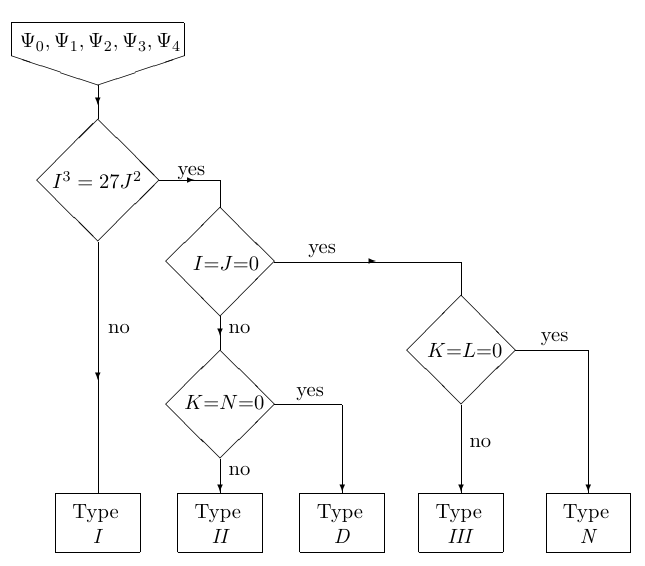
\includegraphics[width=0.7\linewidth]{Figures/Ch5/petrov scheme.png}
    \caption{Petrov classification based on scalars $\boldsymbol{\psi_{0-4}}$}
    \label{petrov classification}
\end{figure}($\boldsymbol{\psi_0}$,$\boldsymbol{\psi_1}$,$\boldsymbol{\psi_2}$,$\boldsymbol{\psi_3}$,$\boldsymbol{\psi_4}$) 
\begin{equation}
    \boldsymbol{\psi_0} = C_{\mu \nu \sigma \rho}k^{\mu}m^{\nu}k^{\sigma}m^{\rho},
    \notag
\end{equation}
\begin{equation}
    \boldsymbol{\psi_1} = C_{\mu \nu \sigma \rho}k^{\mu}l^{\nu}k^{\sigma}m^{\rho},
    \notag
\end{equation}
\begin{equation}
    \boldsymbol{\psi_2} = C_{\mu \nu \sigma \rho}k^{\mu}m^{\nu}\Bar{m}^{\sigma}l^{\rho},
    \label{psies classificaione petrov}
\end{equation}
\begin{equation}
    \boldsymbol{\psi_3} = C_{\mu \nu \sigma \rho}l^{\mu}k^{\nu}l^{\sigma}\Bar{m}^{\rho},
    \notag
\end{equation}
\begin{equation}
    \boldsymbol{\psi_4} = C_{\mu \nu \sigma \rho}l^{\mu}\Bar{m}^{\nu}l^{\sigma}\Bar{m}^{\rho}.
    \notag
\end{equation}
Finally we define some new quantities as 
\begin{align}
    I & = \boldsymbol{\psi_0}\boldsymbol{\psi_4}-4\boldsymbol{\psi_1}\boldsymbol{\psi_3}+3\boldsymbol{\psi_2}^2 , & J &= \det \left(\begin{matrix}
    \boldsymbol{\psi_0} & \boldsymbol{\psi_1} & \boldsymbol{\psi_2} \\
    \boldsymbol{\psi_1} & \boldsymbol{\psi_2} & \boldsymbol{\psi_3} \\
    \boldsymbol{\psi_2} & \boldsymbol{\psi_3} & \boldsymbol{\psi_4} \\
\end{matrix} \right) 
\label{quantità di petrov 1}
\end{align}
\begin{align}
  K & = \boldsymbol{\psi_1}\boldsymbol{\psi_4}^2-3\boldsymbol{\psi_4}\boldsymbol{\psi_3}\boldsymbol{\psi_2} +2\boldsymbol{\psi_3}^3 ,& L &= \boldsymbol{\psi_2}\boldsymbol{\psi_4}-\boldsymbol{\psi_3}^2 ,&
  N& = 12L^2-\boldsymbol{\psi_4}^2I.
  \label{quantità di petrov 2}
\end{align}
To label a metric with Petrov classification we can easily follow the scheme in figure \ref{petrov classification} based on quantities (\ref{quantità di petrov 1})-(\ref{quantità di petrov 2}).
If we take the BBMB solution with the tetrad (\ref{tetrad assiale generale}) this leads to $\boldsymbol{\psi_1}=\boldsymbol{\psi_3}=0$, $\boldsymbol{\psi_0}=\boldsymbol{\psi_4}=3\boldsymbol{\psi_2}$ and $\boldsymbol{\psi_2}=\frac{m(m-r)}{2r^4}$, so looking at scheme \ref{petrov classification}, BBMB is clearly a Type D solution. Contrary, if we consider solution (\ref{BBMB+VIII)}) with the same tetrad, after a bit of calculation to evaluate the scalars, we can easily see that $I^3-27J^2\neq 0$, so we have a Type I solution.

\section{Applying transformation VIII to RNS black hole} \label{Capitolo RNS + VIII}
We can repeat the same procedure for the RNS solution with little effort. The result will be a new solution with constant scalar field since, as seen in the previous section, this transformation is non trivial.
The RNS solution in spherical coordinates appear as 
\begin{equation}
    ds^2 = -\left(1 -\frac{2m}{r}+\frac{s+e^2}{r^2} \right) dt^2 + \left(1 -\frac{2m}{r}+\frac{s+e^2}{r^2} \right)^{-1} dr^2 + r^2\left(d\theta^2+\sin^2\theta d\varphi^2\right),
    \label{Reissner nordstrom peloso sferiche}
\end{equation}
\begin{equation}
    \psi = \sqrt{\frac{6}{k}}\sqrt{\frac{s}{s+e^2}}
    \notag
\end{equation}
with $\Bar{A} = -\frac{e}{r} dt$. We can map the conformal LWP ansatz into (\ref{Reissner nordstrom peloso sferiche}) with the change of coordinates
\begin{equation*}
    \begin{aligned}
        \begin{cases}
           \rho  = \sqrt{Q(r)}\sin\theta \\
           z = (r-m)\cos\theta \\
           \varphi = \varphi \\
        \end{cases}
    \end{aligned}
    \label{cambio cilindriche sferiche reissner nordstrom}
\end{equation*}
where $Q(r)\equiv r^2-2mr+e^2+s$, so that 
\begin{equation}
    d\rho^2 + dz^2 = (r^2-2mr+m^2\sin^2\theta+(e^2+s)\cos^2\theta)\left(\frac{dr^2}{Q(r)} + d\theta^2\right)
    \notag
\end{equation}
and with the identifications 
\begin{equation*}
    \begin{aligned}
        \begin{cases}
           \displaystyle f  = 1-\frac{2m}{r}+\frac{e^2+s}{r^2} \\[0.5em] 
           \displaystyle e^{2\gamma} = \frac{Q(r)}{r^2-2mr+m^2\sin^2\theta+(e^2+s)\cos^2\theta} \\
           \displaystyle Q(r) = r^2-2mr+e^2+s \\
        \end{cases}
        \begin{cases}
            \omega = 0 \\
            \Omega = 1 \\
            \displaystyle \chi = \frac{-3e^2}{s+e^2}. \\
        \end{cases}
    \end{aligned}
\end{equation*}
From this, the transformation VIII becomes
\begin{align}
        &\chi \rightarrow \chi' = 3\left(\tanh^2\left[\frac{l}{2}\log\left[\frac{-3 e^2\sqrt{Q(r)}}{s+e^2}\sin\theta\right] \pm \operatorname{arctanh} \left[ \sqrt{\frac{s}{s+e^2}}\right]\right] - 1\right), \notag\\[0.5em]
        &\gamma \rightarrow \gamma' = \gamma + 3l\left(\frac{l}{4}\log\left[\frac{-3 e^2\sqrt{Q(r)}}{s+e^2}\sin\theta\right] \pm \operatorname{arctanh} \left[ \sqrt{\frac{s}{s+e^2}}\right] \right).\notag
\end{align}
In this case as well, we have to impose $\Omega' = \chi/\chi'$. Finally the transformed solution reads as 
\begin{equation}
    ds^2=\Omega'\left[-\frac{Q(r)}{r^2}dt^2+r^2\left(\frac{dr^2}{Q(r)} + d\theta^2 \right) e^{6l(\xi-\eta)}+r^2\sin^2\theta d\varphi^2\right],
    \notag
\end{equation}
\begin{equation}
    \psi=\sqrt{\frac{6}{k}}\sqrt{1-\operatorname{sech}^2\xi} 
    \label{R.N. PELOSO +VIII)}
\end{equation}
where
\begin{equation}
    \xi = 2\eta \pm \operatorname{arctanh} \left[ \sqrt{\frac{s}{s+e^2}}\right], \notag
\end{equation}
\begin{equation}
    \eta = \frac{l}{4}\log\left[\frac{-3 e^2\sqrt{Q(r)}}{s+e^2}\sin\theta\right], \notag
\end{equation}
\begin{equation}
    \Omega' = \frac{-e^2}{( \tanh^2\xi-1)(s+e^2)} \notag
\end{equation}
with $l \in \mathbb{R}$ and the electromagnetic potential that remains unchanged $\Bar{A} = -\frac{e}{r} dt$. Using the same Newman-Penrose tetrad from the previous section, this solution turns out to be a Petrov Type I.

% \section{Applying transformation XI to RNS black hole} \label{capitolo rns + XI}
% The last of the new symmetry that we apply is transformation XI on RNS solution. This involves the coordinate $\rho$, so it is convenient to remain in cylindrical coordinates despite the spherical symmetry of the metric. From \citep{Emparan_Teo} we know that a generic solution of the form
% \begin{equation}
%     ds^2 = -\frac{r^2-2mr+q^2}{r^2}dt^2+\frac{r^2}{r^2-2mr+q^2}dr^2+r^2(d\theta^2+\sin^2\theta d\varphi^2)
%     \notag
% \end{equation}
% with $A_t=-q/r$ and related to cylindrical coordinates as 
% \begin{equation*}
%     \begin{aligned}
%         \begin{cases}
%            \rho  = \sqrt{r^2-2mr+q^2}\sin\theta \\
%            z = (r-m)\cos\theta \\
%         \end{cases}
%     \end{aligned}
%     \notag
% \end{equation*}
% can be rewritten in term of the LWP metric with 
% \begin{equation}
%     f_0 = \frac{(R_+^0+r_+^0)^2-4(m^2-q^2)}{(R_+^0+r_+^0+2m)^2}
% \end{equation}
% \begin{equation}
%     e^{2\gamma_0} = \frac{(R_+^0+r_+^0)^2-4(m^2-q^2)}{4R_+^0r_+^0}
% \end{equation}
% \begin{equation}
%     A_{t_0} = \frac{-2q}{R_+^0+r_+^0+2m}
% \end{equation}
% and 
% \begin{equation}
%     R_+^0=\sqrt{\rho^{2}+(z+\sqrt{m^2-q^2})}
% \end{equation}
% \begin{equation}
%     r_+^0=\sqrt{\rho^{2}+(z-\sqrt{m^2-q^2})}
% \end{equation}
% From this, we can easily convert it to our case with\footnote{For the electromagnetic potential $A_t$ we have to substitute just $e$ instead of $\sqrt{e^2+s}$, since without electric charge the potential must vanishes.} $q^2=e^2+s$ and then apply the transformation $\rho \rightarrow \rho^p\alpha^{p-1}$, $\gamma_0\rightarrow \gamma / p$ so that the solution becomes
% \begin{equation}
%     ds^2=-fdt^2 + f^{-1}\left[e^{2\gamma}(dz^2+p^2(\alpha\rho)^{2p-2}d\rho^2)+\rho^{2p}\alpha^{2p-2}d\varphi^2\right]
%     \label{RNS + XI}
% \end{equation}
% \begin{align}
%   \psi & = \sqrt{\frac{6}{k}}\sqrt{\frac{s}{s+e^2}} & \Bar{A} &= A_t dt  
% \end{align}
% where 
% \begin{equation}
%     R_+=\sqrt{\rho^{2p}\alpha^{2p-2}+(z+\sqrt{m^2-e^2-s})}
% \end{equation}
% \begin{equation}
%     r_+=\sqrt{\rho^{2p}\alpha^{2p-2}+(z-\sqrt{m^2-e^2-s})}
% \end{equation}
% \begin{equation}
%     f = \frac{(R_++r_+)^2-4(m^2-e^2-s)}{(R_++r_++2m)^2}
% \end{equation}
% \begin{equation}
%     e^{2\gamma} = \left[\frac{(R_++r_+)^2-4(m^2-e^2-s)}{4R_+r_+}\right]^{1/p}
% \end{equation}
% \begin{equation}
%     A_t = \frac{-2e}{R_++r_++2m}
% \end{equation}
% \begin{equation}
%     \alpha = \chi =4\pi\psi^2-3= \frac{-3e^2}{s+e^2}
% \end{equation}
% Clearly with $p=1$ we recover the seed solution, while for $p\notin \mathbb{N}$ we must impose $s<-e^2$ so that $\alpha>0$.